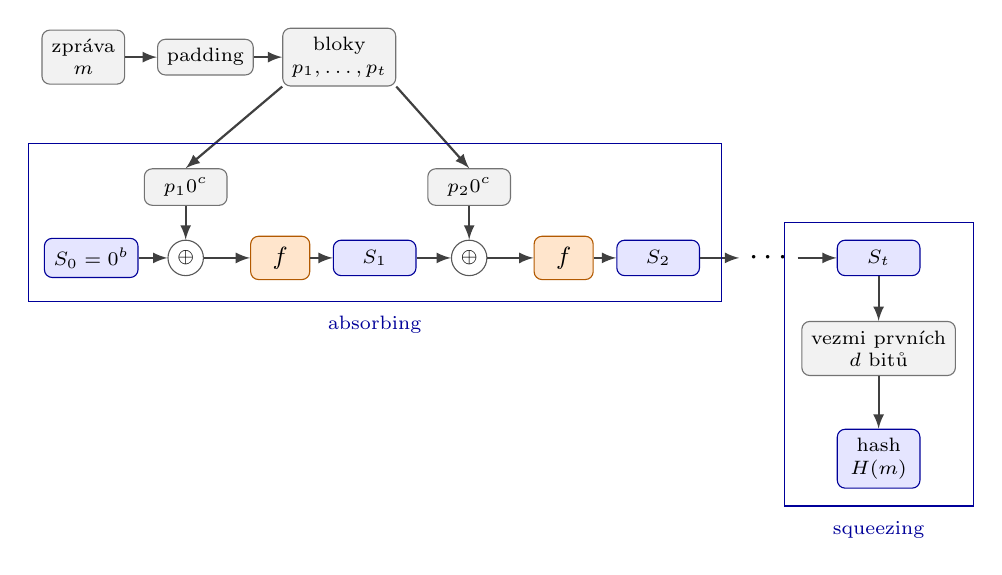
\begin{tikzpicture}[
    x=1cm,y=1cm,
    >=latex,
    block/.style={
        rounded corners=1mm,
        draw=black!55,
        fill=black!5,
        minimum width=1.05cm,
        minimum height=0.45cm,
        font=\scriptsize,
        align=center
    },
    state/.style={
        rounded corners=1mm,
        draw=blue!60!black,
        fill=blue!10,
        minimum width=1.05cm,
        minimum height=0.45cm,
        font=\scriptsize,
        align=center
    },
    func/.style={
        rounded corners=1mm,
        draw=orange!70!black,
        fill=orange!20,
        minimum width=0.75cm,
        minimum height=0.55cm,
        font=\small\bfseries,
        align=center
    },
    arr/.style={->, >=latex, line width=0.8pt, draw=black!75},
    xor/.style={
        circle,
        draw=black!65,
        fill=white,
        minimum size=4.5mm,
        inner sep=0pt,
        font=\scriptsize
    }
]

    % input
    \node[block] (M) at (-5.1,2.1) {zpráva\\ \(m\)};
    \node[block] (pad) at (-3.55,2.1) {padding};
    \node[block] (split) at (-1.85,2.1) {bloky\\ \(p_1,\ldots,p_t\)};

    \draw[arr] (M) -- (pad);
    \draw[arr] (pad) -- (split);

    % state chain
    \node[state] (S0) at (-5.0,-0.45) {\(S_0=0^b\)};
    \node[xor] (xor1) at (-3.8,-0.45) {\(\oplus\)};
    \node[func] (f1) at (-2.6,-0.45) {\(f\)};
    \node[state] (S1) at (-1.4,-0.45) {\(S_1\)};

    \node[xor] (xor2) at (-0.2,-0.45) {\(\oplus\)};
    \node[func] (f2) at (1.0,-0.45) {\(f\)};
    \node[state] (S2) at (2.2,-0.45) {\(S_2\)};

    \node[font=\large] (dots) at (3.6,-0.45) {\(\cdots\)};

    \node[state] (St) at (5.0,-0.45) {\(S_t\)};

    \draw[arr] (S0) -- (xor1);
    \draw[arr] (xor1) -- (f1);
    \draw[arr] (f1) -- (S1);
    \draw[arr] (S1) -- (xor2);
    \draw[arr] (xor2) -- (f2);
    \draw[arr] (f2) -- (S2);
    \draw[arr] (S2) -- (dots);
    \draw[arr] (dots) -- (St);

    % input blocks to xor
    \node[block] (P1) at (-3.8,0.45) {\(p_1 0^c\)};
    \node[block] (P2) at (-0.2,0.45) {\(p_2 0^c\)};
    \draw[arr] (P1) -- (xor1);
    \draw[arr] (P2) -- (xor2);
    \draw[arr] (split.south west) -- (P1.north);
    \draw[arr] (split.south east) -- (P2.north);

    % squeezing
    \node[block] (out) at (5.0,-1.60) {vezmi prvních\\ \(d\) bitů};
    \node[state] (hash) at (5.0,-3.00) {hash\\ \(H(m)\)};

    \draw[arr] (St) -- (out);
    \draw[arr] (out) -- (hash);

    % labels
    \node[font=\scriptsize, text=blue!60!black] at (-1.4,-1.3) {absorbing};
    \draw[draw=blue!60!black] (-5.8,1.0) rectangle (3.0,-1.0);
    \node[font=\scriptsize, text=blue!60!black] at (5.0,-3.9) {squeezing};
    \draw[draw=blue!60!black] (3.8,0) rectangle (6.2,-3.6);

\end{tikzpicture}
